\begin{figure}[htbp]
  \centering
  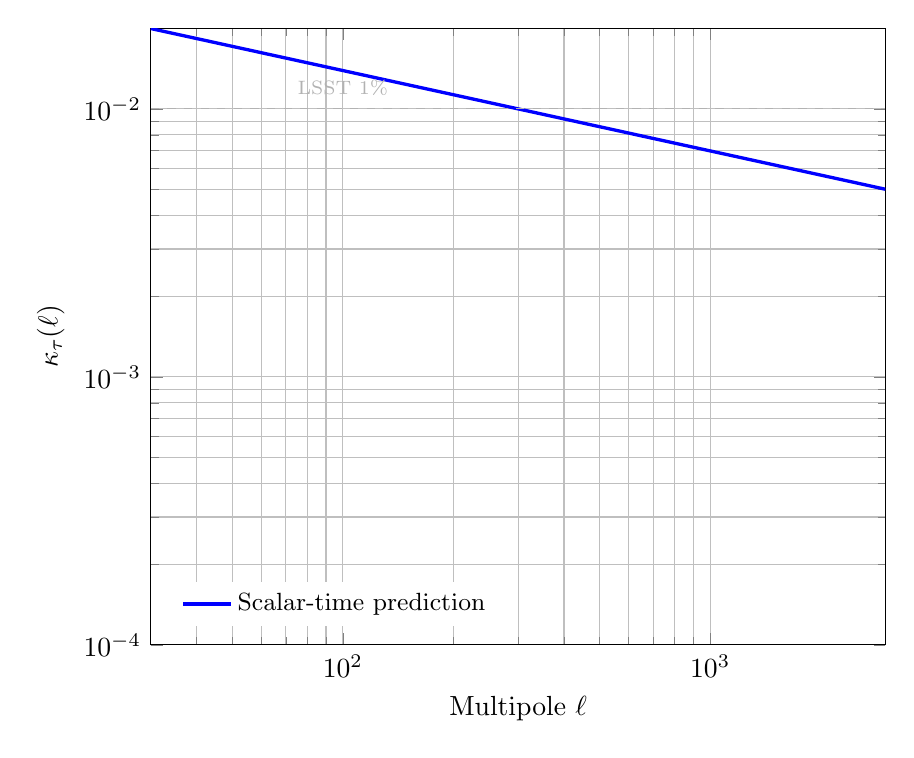
\begin{tikzpicture}
  \begin{axis}[
      width=0.9\textwidth,
      xlabel={Multipole $\ell$},
      ylabel={$\kappa_{\tau}(\ell)$},
      xmode=log, ymode=log,
      xmin=30,  xmax=3000,
      ymin=1e-4, ymax=2e-2,
      grid=both,
      legend style={draw=none, font=\small},
      legend pos=south west]
    %
    % κ_tau ∝ (ℓ/300)^(-0.3) scaled to 1 % at ℓ = 300
    \addplot[very thick,blue,domain=30:3000,samples=250]
      {0.01*pow(x/300,-0.3)};
    \addlegendentry{Scalar-time prediction}
    %
    % horizontal 1% LSST sensitivity line
    \addplot[gray!60,dashed] coordinates {(30,0.01) (3000,0.01)};
    \node[gray!60] at (axis cs:100,0.012) {\scriptsize LSST 1\%};
  \end{axis}
  \end{tikzpicture}
  %-------------------------------------------------------------
  \caption{Predicted weak-lensing convergence residual $\kappa_{\tau}$ for the scalar-time model.  The signal peaks at $\ell\!\approx\!300$ and stays within the projected 1\,\% statistical sensitivity of Rubin LSST (dashed line) across a broad range of scales.}
  \label{fig:WeakLensing}
\end{figure}
